\section{STANDARD PROCESS MODEL FOR DATA MINING (CRISP-DM)}

Según \parencite{wirth2000crisp} la metodología \textit{CRISP-DM} proveé una visión general del ciclo de vida de un proyecto basado en \textit{Minería de Datos}. Este ciclo de vida se descompone en seis fases: \textit{Entendimiento del Negocio}, \textit{Entendimiento de los Datos}, \textit{Preparación de los Datos}, \textit{Modelado}, \textit{Evaluación} y \textit{Despliegue}. Estas fases siguen un proceso secuencial no estricto y se puede adaptar a las necesidades del proyecto, sin embargo, existe una secuencia frecuente basada en las dependencias de cada fase.

En el contexto del proyecto actual, las metodologías basadas en Minería de Datos deben ser tomadas en cuenta debido a que los Sistemas de Recomendación forman parte del ámbito de dicha disciplina y, \textit{CRISP-DM} ha sido diseñado para estructurar proyectos de Minería de Datos sin establecer un objetivo en específico (clasificación, clustering, regresión, recomendación).

\begin{figure}[h!]
    \centering
    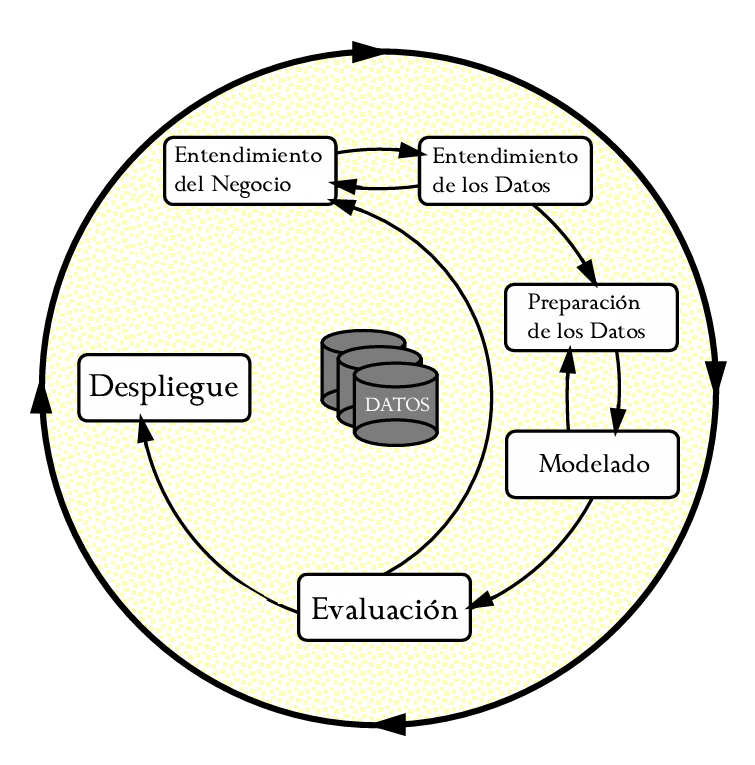
\includegraphics[width=0.65\linewidth]{CRISPDM.png}
    \caption{Fases de la Metodología CRISP-DM \parencite{wirth2000crisp}.}
    \label{fig:FasesCRISPDM}
\end{figure}

En la figura \Cref{fig:FasesCRISPDM} se puede visualizar que las fases de \textit{CRISP-DM} son cíclicas debido a la naturaleza de la \textit{Minería de Datos}, ya que estos se retroalimentan de sus propios resultados, ya sean errores o aciertos.

Cada una de las fases que componen a la metodología \textit{CRISP-DM} cumplen con un propósito específico, a continuación se describe la función de cada una de las fases.

\subsection{FASE 1: ENTENDIMIENTO DEL NEGOCIO}
La fase inicial denominada como \textit{Entendimiento del Negocio} se enfoca en entender los objetivos y requerimientos del proyecto, convirtiéndo este conocimiento en la definición de un problema a resolver mediante \textit{Minería de Datos} y en un plan de proyecto preliminar diseñado para cumplir dichos objetivos.

La situación del negocio debe ser evaluada para obtener una visión general de los recursos necesarios. Uno de los puntos más importantes de esta fase es la determinación del \textbf{Objetivo de la Minería de Datos}. El primer paso es definir el tipo de Minería de Datos que se desarrollará (en este caso, Recomendación) y el criterio de éxito \parencite{schroer2021systematic}. 

Según \parencite{wirth2000crisp}, esta fase está compuesta de tareas específicas que ayudan a cumplir su funcionamiento:

\begin{enumerate}
    \item \textbf{Determinar los Objetivos del Negocio: } Tomando en cuenta el contexto y los criterios de éxito. 
    \item \textbf{Evaluar la Situación:} Definiendo los recursos de inventario, requerimientos, riesgos y contingencias, costos y beneficios.
    \item \textbf{Determinar los Objetivos de la Minería de Datos:} Considerando los criterios de éxito de éste proceso.
    \item \textbf{Producir un Plan de Proyecto:} Y tomar en cuenta una evaluación inicial de las herramientas y técnicas a usar.
\end{enumerate}

\subsection{FASE 2: ENTENDIMIENTO DE LOS DATOS}
La fase de \textit{Entendimiento de los Datos} empieza con una colección de datos inicial y es seguida de actividades que fomenten el entendimiento de los datos para identificar problemas de calidad, descubrir perspectivas iniciales o detectar subcolecciones para identificar información escondida.

Esta fase se compone de las siguientes actividades \parencite{wirth2000crisp}:

\begin{enumerate}
    \item \textbf{Recolectar los Datos Iniciales: } Forjando una colección inicial de los datos.
    \item \textbf{Describir los Datos: } Elaborar un reporte enfocado a describir los datos obtenidos.
    \item \textbf{Explorar los Datos: } Elaborar un reporte de exploración de los datos.
    \item \textbf{Verificar la Calidad de los Datos: } Y elaborar un reporte de la calidad de los datos.
\end{enumerate}

\subsection{FASE 3: PREPARACIÓN DE LOS DATOS}

La fase de \textit{Preparación de los Datos} se enfoca en construir el \textit{Dataset} final en base a la primera recolección de datos. Estas tareas de preparación se deben ejecutar múltiples veces. Estas actividades incluyen tareas de selección de tablas, limpieza de datos, construcción de nuevos atributos y transformación de datos para herramientas de modelado.

Además, se debe realizar un proceso de selección de datos definiendo criteros de inclusión y exclusión. Los datos de mala calidad deben ser procesados mediante una tarea de limpieza de datos \parencite{schroer2021systematic}.

Las actividades específicas de esta fase son las siguientes:

\begin{enumerate}
    \item \textbf{Establecer el Dataset Final: } Además de elaborar una descripción detallada.
    \item \textbf{Seleccionar los Datos: } A través de criterios de inclusión y exclusión.
    \item \textbf{Limpieza:} Limpiar los datos de mala calidad y reportar los cambios.
    \item \textbf{Construcción:} Construir los datos mediante nuevos atributos y generar registros manuales de simulación o de entrenamiento.
    \item \textbf{Integrar los Datos:} Fusionar los nuevos datos con los previamente existentes.
    \item \textbf{Reformatear: } Establecer un formato específico para los datos.
\end{enumerate}

\subsection{FASE 4: MODELADO}

